\documentclass[letterpaper]{article}

% authors and affiliations
\title{PMoveSTIR---A general framework to incorporate movement and space use information in epidemiological models}
\usepackage{authblk}
\author{Juan S. Vargas Soto \and Mark Q. Wilber}
\affil{School of Natural Resources, University of Tennessee, Knoxville, TN}
\date{}


\usepackage[english]{babel}
\usepackage[utf8x]{inputenc}
\usepackage{amsmath}
\usepackage{graphicx}
\usepackage[left=1 in, right=1 in, top=1 in, bottom=1 in]{geometry}
\usepackage{hyperref}
\usepackage{bbold}
\usepackage{rotating}
\usepackage{bbm}
\usepackage{array}
\usepackage{xcolor}
\newcolumntype{C}[1]{>{\centering\arraybackslash}m{#1}}
% \usepackage{kbordermatrix}
\usepackage{footnote}
\makesavenoteenv{tabular}
\makesavenoteenv{table}
% \renewcommand{\theequation}{{S}\arabic{equation}}

\makeatletter
% \addto\captionsenglish{%
%   \renewcommand{\fnum@figure}{Figure S\thefigure}%
%   \renewcommand{\fnum@table}{Table S\thetable}%
% }
\makeatother

% Bibliography
\usepackage[round, colon]{natbib} % Bibliography - APA
\bibliographystyle{abbrvnat}
%\bibpunct{(}{)}{;}{a}{}{,}

% Line numbers
\usepackage{lineno}
%\def\linenumberfont{\normalfont\footnotesize\ttfamily}
%\setlength\linenumbersep{0.2 in}
\linenumbers

% Set space
\usepackage{setspace}
\doublespacing

% Command to e.g. write code that doesn't show up. Used as \ignore {some code}
\newcommand{\ignore}[1]{}

\begin{document}

\maketitle

\section*{Introduction}

Individual movement is among the most critical factors that determine the dynamics of infectious disease in wildlife \citep{Manlove2022,Dougherty2022}. 
%For example, the combined dispersal of individuals in a population defines how parasites and infectious diseases spread across the landscape \citep{Fofana2017}. 
%At a more local scale, 
From an individual perspective, how an animal moves determines whether they encounter other individuals of the same species, other species, or parasites in the environment. 
These encounters are a necessary component for parasite transmission, and efforts have sought to identify where they could occur, how often, and how they could be influenced by environmental drivers. 
Being able to formally link environmental factors, animal movement, contact, and parasite transmission risk, could improve our ability to predict and prevent outbreaks and would represent a significant advancement for management of wildlife diseases.  
Nevertheless, understanding and extrapolating the relationships between these processes at an individual scale requires extremely detailed information about movement, combined with analytical frameworks that can translate this information into an epidemiological context.

Recent approaches developed at the interface of movement and disease ecology are able to leverage animal tracking data with high spatial and temporal resolution to gain insight into contact among individuals and disease transmission \citep{Wilber2022,Yang2023}. For example, movement-driven modeling of spatio-temporal infection risk (MoveSTIR) builds dynamic spatio-temporal contact networks from which we can estimate the risk of infection for different individuals across space and time \citep{Wilber2022}. MoveSTIR provides a theoretical foundation to translate contacts observed or inferred from spatial data into the epidemiological currency of force of infection, which represents the risk of transmission experienced by a host per unit time. These studies have highlighted the importance of individual heterogeneity and temporal scale for disease dynamics, particularly how indirect contact---two individuals at the same place at different times---can significantly reshape contact and transmission networks \citep{Wilber2022,Yang2023}. This framework is nonetheless based on occurrence, rather than range, distributions \citep[in the terminology of ][]{Alston2022} -- meaning it only considers where animals were observed and not where they \emph{potentially} could have moved. This makes it difficult to systematically link observed encounters with underlying spatial covariates, and to predict how social or environmental changes affect contact and transmission. 

An alternative approach would be to use utilization distributions (UDs) to infer spatial and temporal contact and transmission in a probabilistic way. An individual's UD is defined as the probability--either transient or in the long-run \citep{Tao2016}--that it uses a particular area on a landscape, and is perhaps the best representation of the long-term relationship between spatial environment and spatial phenotype [\textcolor{blue}{COMMENT: What do you mean by spatial phenotype?}] over different time scales \citet{Webber2023}. The high spatial and temporal resolution of modern tracking data serves to build UDs based on biologically realistic movement models \citep{Fleming2014,Gurarie2011,Potts2023}, and to link them with underlying resources.
Individually defined UDs can be combined to study pairwise interactions, for example to quantify the degree of overlap between home ranges \citep{Winner2018}, or to estimate the expected location and rate of encounter between individuals  \citep{Noonan2021}, which could be used to infer contact and transmission \citep{Godfrey2010, Godfrey2013}. 
Moreover, because UDs can be directly linked to environmental drivers of movement \citep{Signer2017}, they have the potential to predict contact and transmission in novel environments and can also be used for prospective analyses to understand how the effects of environmental and social perturbations cascade across scales, from individual movement to population and landscape-level disease transmission. 

Current contact metrics based on UDs focus only on direct interaction, ignoring temporal dynamics that are especially relevant for epidemiological processes. The Conditional Distribution of Encounters (CDE) \citep{Noonan2021}, for example, estimates the probability that two individuals will come into contact with each other at a given location, assuming that individuals move independently from each other.
While a useful simplification, social interactions like territoriality or gregariousness can invalidate this assumption  \citep{Manlove2018,Sah2018}. In these cases, temporal correlations in space use could increase or decrease the expected probability of encounter compared to an assumption of independent movement. 
Moreover, direct interactions do not necessarily equate to \emph{epidemiological contacts}, which consist of contact formation, contact duration, pathogen acquisition, pathogen shedding, and pathogen decay. As some parasites can persist in the environment for months or years (e.g. anthrax, CWD), ignoring these processes could severely underestimate the risk of transmission \citep{Wilber2022,Yang2023,Richardson2015}.

In general, we lack a way to quantify the role of social interactions on spatio-temporal force of infection, which limits our ability to assess whether ignoring correlated movements actually matters when assessing infection risk. One of our goals in this study is to ask: how much can correlated, social movements affect spatio-temporal infection risk? A large portion of epidemiological theory is built upon the assumption of independent host movements in the presence of absence of spatial heterogeneity, but there is very little work that quantifies how correlated movements affect contact and transmission risk. While MoveSTIR implicitly accounts for such correlations, it only applies for observed data. In contrast, the CDE provides a basis for estimating encounter probabilities across the landscape, but ignores correlations and temporal dynamics of indirect contact.
Ultimately, an approach is needed that combines the range-distribution inference of UDs and CDEs \citep{Alston2022,Noonan2021} with the epidemiological focus of MoveSTIR to link UDs to epidemiological dynamics. 

Here, we develop a model we refer to as Probabilistic MoveSTIR (PMoveSTIR) to estimate epidemiological contact and expected force of infection across space and time from UDs. Our approach provides probabilistic, spatio-temporal contact networks that can be used to predict out-of-sample transmission risk under independent or correlated movements \textcolor{blue}{COMMENT: Can we do out-of-sample prediction of correlated movement? We would need an extrapolated or interpolated surface for this.}. We first derive the most general PMoveSTIR model using transient UDs and then show how under assumptions of statistical stationarity and independent movements PMoveSTIR is proportional to the CDE (but represents transmission risk in the units of force of infection). We also show how PMoveSTIR encompasses other common assumptions such as mass action transmission and home range overlap transmission as special cases. Deriving analytical results and applying PMoveSTIR to simulated movement data, we demonstrate the sometimes sizable importance of non-independent movements on pairwise transmission risk, indicating that ignoring the social drivers of contact could severely bias epidemiological inference. However, our simulations show that this result primarily holds for directly transmitted parasites and for parasites that persist for long periods of time in the environment, non-independent host movements are largely inconsequential compared to spatial overlap for transmission risk. We demonstrate this result empirically using a dataset of white-tail deer movements and show that empirically observed correlated movements can increase potential force of infection by orders of magnitude for a hypothetical directly transmitted parasite but are relatively unimportant for a hypothetical parasite with longer persistence times.  Overall, PMoveSTIR is a critical next step for developing predictive models that link movement data to spatio-temporal infection dynamics on real landscapes.

\section*{Methods}

\subsection*{Model development - Linking utilization distributions to transmission through PMoveSTIR}

The PMoveSTIR approach builds on the recently developed MoveSTIR model \citep{Wilber2022} and formally links host utilization distributions, direct and indirect contacts, correlated animal movements, and spatial estimates of force of infection (FOI). This an essential quantity in disease ecology that underlies our ability to predict the spread of disease across populations and landscapes. Essentially, we want to know, for two individuals $i$ and $j$ moving and interacting across a landscape, what is the FOI host $i$ experiences from host $j$, across space and time?  

As in MoveSTIR, we assume that transmission happens by an infected host depositing pathogen into the environment and another host picking that pathogen up. 
Deposition and acquisition can represent a range of processes, from one individual coughing and another inhaling in a matter of seconds, to one host depositing parasite eggs or larvae in the environment and another individual consuming these  days or weeks later. 
This fairly general assumption encompasses standard density-dependent transmission as a special case \citep{Cortez2021}. 
Moreover, considering transmission through deposition and acquisition components clearly links direct transmission and indirect transmission along a continuum \citep{Wilber2022}.
We interpret that a ``contact'' can occur if both individuals visit a given location $x$, which could be a habitat patch or a grid cell. 
Importantly, we assume that locations $x$ on the landscape do not overlap such that summing the areas of locations $x$ equals some total area over which individuals can move (see SI for a derivation when $x$ is a point, not an area, on the landscape). 
Furthermore, we assume that the likelihood of contact is uniform within the location $x$, consistent with a so-called top hat encounter function \citep{Gurarie2013,Wilber2022}.

Given these assumptions, we can define the pairwise force of infection felt by host $i$ from host $j$ in location $x$ at time $t$ as \citep{Wilber2022}
\begin{equation}
    h_{i \leftarrow j}(t, x) = \int_{-\infty}^{t} \beta' \lambda \delta_{x_j(u)}(x) \delta_{I_j(u)}(I) S(t - u) du
    \label{eq:original_foi}
\end{equation}
where $\lambda$ is the pathogen deposition rate of host $j$, $\delta_{x_j(u)}(x)$ is an indicator variable that is one if host $j$ is in location $x$ at time $u$ and zero otherwise, $\delta_{I_j(u)}(I)$ is an indicator function that is one if host $j$ is in an infected state at time $u$ and zero otherwise, and $S(t-u)$ is the probability that any pathogen deposited at time $u < t$ is still alive at time $t$ \citep[see][for a full derivation]{Wilber2022}.  
The term $\beta'$ is the rate at which host $i$ picks up pathogen within the location $x$ and can be re-written as $\tilde{\beta} / A_x$, where $\tilde{\beta}$ can be considered a ``search efficiency'' term, with units area/time (e.g., $m^2 / day$), and $A_x$ gives the area of location $x$ (e.g., 100 $m^2$). 
Therefore, the total acquisition rate scales with the area in which contact can occur; in larger areas, the acquiring host would have to search for longer to find a ``packet'' of pathogen, reducing the host's total acquisition rate and the corresponding FOI. 
%The same amount of pathogen spread over a larger area would reduce the total acquisition rate .  deposited by host $j$  (or, equivalently, host $i$ would have to traverse a larger area ),  .  
%As we derive PMoveSTIR, it is critical to be specific about our definition of contact and the area units associated with $\beta'$.

Moving forward, we will make an assumption of maximum transmission risk and assume that host $j$ (the depositing host) is always infected. 
This is equivalent to building a contact network and also represents the structural form of FOI needed to compute pathogen invasion thresholds \citep{Wilber2022}.
Considering probabilistic movements, we can then re-write equation \ref{eq:original_foi} as
\begin{equation}
    h_{i \leftarrow j}(t, x) = \int_{-\infty}^{t} \beta' \lambda \delta'_{x_i(t)}(x) \delta'_{x_j(u)}(x) S(t - u) du
    \label{eq:prob_foi}
\end{equation}
where $\delta'_{x_i(t)}(x)$ and $\delta'_{x_j(u)}(x)$ are random variables that specify whether or not (i.e., 0 or 1) host $i$ or host $j$ is in location $x$ at time $t$.  This means that $h_{i \leftarrow j}(t, x)$ is also a random variable, and we can express its expected value as 
\begin{equation}
    E[h_{i \leftarrow j}(t, x)] := h^*_{i \leftarrow j}(t, x) = \int_{-\infty}^{t} \beta' \lambda E[\delta'_{x_i(t)}(x) \delta'_{x_j(u)}(x)] S(t - u) du.
    \label{eq:expected_foi}
\end{equation}
Interpreting this expectation, we are asking: if we simulated some movement process thousands of times, what is the probability that host $i$ is in location $x$ at time $t$ and host $j$ was in location $x$ at a previous time $u$? 

\subsubsection*{Linking equation \ref{eq:expected_foi} to utilization distributions}

%Our goal is to understand how utilization distributions link to spatio-temporal transmission risk. 
Note that for two random variables $Y$ and $Z$, we have $E[YZ] = E[Y]E[Z] + Cov(Y, Z)$.  We can therefore write equation \ref{eq:expected_foi} as

\begin{equation}
    \begin{aligned}
        h^*_{i \leftarrow j}(t, x) &= \int_{-\infty}^{t} \frac{\tilde{\beta}}{A_x} \lambda E[\delta'_{x_i(t)}(x) \delta'_{x_j(u)}(x)] S(t - u) du \\
        &= \frac{\tilde{\beta}}{A_x} \lambda \int_{-\infty}^{t} [E[\delta'_{x_i(t)}(x)] E[\delta'_{x_j(u)}(x)] + Cov(\delta'_{x_i(t)}(x), \delta'_{x_j(u)}(x))] S(t - u) du \\
        &= \frac{\tilde{\beta}}{A_x} \lambda \int_{-\infty}^{t} [p_i(x, t) p_j(x, u) + Cov(\delta'_{x_i(t)}(x), \delta'_{x_j(u)}(x))] S(t - u) du \\
    \end{aligned}
    \label{eq:foi_cov}
\end{equation}
where we use the fact that the expectation of an indicator variable is a probability \citep{Grimmett2001}. The terms $p_i(x, t)$ and $p_j(x,u)$ give the probabilities that host $i$ and $j$ are in location $x$ at times $t$ and $u$, respectively, and can also be written as $p_i(x, t) = \int_{A_x} f_i(s, t) ds$ where $f_i(s, t)$ is the probability density of host $i$ using the point $s$ at time $t$ and the integral is over the area $A_x$ (defined equivalently for host $j$). Thus, we have obtained an equation that links the transient utilization distributions $f_i(s, t)$ and $f_j(s, u)$ with the spatio-temporal FOI.

% Second, we could write equation \ref{eq:expected_foi} as 

% \begin{equation}
%     \begin{aligned}
%     h^*_{i \leftarrow j}(t, x) &= \int_{-\infty}^{t} \beta' \lambda E[\delta'_{x_i(t)}(x) \delta'_{x_j(u)}(x)] e^{-\nu(t - u)} du \\
%     &= \beta' \lambda \int_{-\infty}^{t} p(i \in x \text{ at } t, j \in x \text{ at } u) e^{-\nu(t - u)} du) \\
%     &= \beta' \lambda \int_{-\infty}^{t} p(i \in x \text{ at } t | j \in x \text{ at } u) p(j \in x \text{ at } u) e^{-\nu(t - u)} du \\
%     \end{aligned}
%     \label{eq:foi_prob}
% \end{equation}



% Instead of assuming hosts are moving uniformly across all $n$ grid cells, assume that they only occupy one grid cell on the landscape.  Now $p_i(x) = p_j(x) = 1$ if $x$ is the grid cell they use and is zero otherwise.  Applying the same steps and summing over all space we get $\frac{\tilde{\beta}}{A_{x}} \frac{\lambda}{\nu}$ -- the FOI from $j$ to $i$ is what we would expect if hosts were moving uniformly over a smaller area $A_x$. 

\subsubsection*{Applying the PMoveSTIR framework under different degrees of spatial and temporal heterogeneity}

Equation \ref{eq:foi_cov} is the most general formulation of PMoveSTIR, where utilization distributions and between-individual spatial covariance are time-varying and heterogeneous in space. For example, this could account for daily changes in habitat use and social interactions. The approach can be modified to consider different degrees of spatial and temporal heterogeneity. This allows us to link FOI to different metrics such as temporally varying utilization distributions, stationary utilization distributions, and home range overlap. Fig. \ref{fig:square} shows the different scenarios that PMoveSTIR can consider. 

In the upper-left corner, we consider space use is uniform, but movement is non-stationary. In this case, it is not important where an individual is, just when. Considering this framing from an empirical point of view, proximity loggers deployed on individual hosts---a commonly used tool to measure among-animal contacts---only tell us when contacts between individuals occur, but not where.  Thus, we cannot make inference about spatial factors driving contacts, but can make inference on temporal processes.  We consider this case in a future study.

In the lower left-hand corner of the PMoveSTIR framework (Fig. \ref{fig:square}), we have the case where space use is uniform and time is stationary. 
Given these assumptions, and the assumption that pathogen decay is exponentially distributed with a rate of decay $\nu$ such that $S(s) = \exp(-\nu s)$, we can write the FOI equation as
\begin{equation}
    \begin{aligned}
        h^*_{i \leftarrow j}(A_x) = \beta' \lambda \left[\frac{A_x}{A_{tot}}\frac{A_x}{A_{tot}} \frac{1}{\nu} +  \int_{0}^{\infty} Cov(\delta_{i \in A_x}, \delta_{j \in A_x} | s) e^{-\nu s} ds\right]
    \end{aligned}
    \label{eq:uniform_stationary1}
\end{equation}
where the covariance in contact is constant across all areas $A_x$ on the landscape (such that $\delta_{i \in A_x}$ indicates the use of some arbitrary area $A_x$).  
If hosts are moving independently (i.e., covariance is 0) we obtain $\frac{\tilde{\beta}}{A_x} \frac{A_x}{A_{tot}} \frac{A_x}{A_{tot}}  \frac{\lambda}{\nu}$. Given a gridded landscape with non-overlapping grids and $x$ is a single grid cell, summing over all $n$ areas $A_x$ that comprise the landscape yields $\bar{h}_{i \leftarrow j} =\frac{\tilde{\beta}}{A_\text{tot}} \frac{\lambda}{\nu}$, which is the standard mass action assumption \citep{McCallum2001}. 

Finally, the lower-right corner represents the special case of statistical stationarity in movement (i.e., the mean location is constant through time, though the animal is still moving).
Again assuming that pathogen survival in the environment follows $S(t - u) = e^{-\nu (t - u)}$, where $\nu$ is a constant pathogen decay rate,  we can simplify equation \ref{eq:foi_cov} to (derivation in SI)
\begin{equation}
    \begin{aligned}
   h^*_{i \leftarrow j}(x) = \frac{\tilde{\beta}}{A_x} \lambda \left[p_i(x)p_j(x) \frac{1}{\nu} + \int_{0}^{\infty} Cov(\delta_{i \in x}, \delta_{j \in x} | \tau) e^{-\nu \tau} d\tau\right]
    \end{aligned}
    \label{eq:foi_stationary}
\end{equation}
The key insight here is that, given a stationarity assumption, the expected force of infection in location $x$ depends on i) the marginal probabilities that host $i$ and host $j$ use location $x$ (i.e. their UDs), 
%, where $p_i(x) = \int_{A_x} f_i(s) ds$ and $p_j(x) = \int_{A_x} f_j(s) ds$ and $f_i$ and $f_j$ are the utilization distributions of host $i$ and $j$ 
and ii) the covariance in how host $i$ and host $j$ use location $x$, integrated over different time lags $\tau$. 
To improve intuition, we can redefine $Cov(\delta_{i \in x}, \delta_{j \in x} | s) = \sigma_i(x) \sigma_j(x) Cor(\delta_{i \in x}, \delta_{j \in x} | s)$, where $\sigma_i(x) = \sqrt{p_i(x)(1 - p_i(x))}$  and $\sigma_j(x) = \sqrt{p_j(x)(1 - p_j(x))}$ are the standard deviation in probability of host $i$ and $j$ using location $x$, respectively.  We can then write
\begin{equation}
    \begin{aligned}
    h^*_{i \leftarrow j}(x) = \beta' \lambda [ \underbrace{p_i(x)p_j(x) \frac{1}{\nu}}_{\substack{\text{FOI contribution from} \\ \text{shared space use}}} + \sigma_i(x) \sigma_j(x) \underbrace{\int_{0}^{\infty} Cor(\delta_{i \in x}, \delta_{j \in x} | \tau) e^{-\nu s} d\tau]}_{\substack{\text{FOI contribution from} \\ \text{correlated movement}}}.
    \end{aligned}
    \label{eq:stationary_cor}
\end{equation}
Equation \ref{eq:stationary_cor} highlights that the key quantity we need to understand is the correlation in host $i$'s and host $j$'s use of location $x$ at different time lags $\tau$, i.e. the temporal cross-correlation in space use.
This correlation is most easily understood for short time lags ($\tau\approx0$), for which a positive value indicates that individuals are at the same location at the same time or one shortly after the other. In contrast, negative correlations at short lags indicate the individuals rarely encounter each other directly.
In what follows, we focus on this case and explore how and under what circumstances correlated movement can influence the FOI. We analyze different scenarios of movement analytically, using simulations, as well as empirical data.  But first, we examine a two additional formulations of PMoveSTIR that highlight the flexibility of this approach for linking range distributions (including home ranges and UDs) and spatial-temporal infection risk.


%Given an assumption of exponential parasite decay, these correlations at short lags also have the greatest effect on the FOI. The effect is nonetheless cumulative, which captures the increase in FOI through prolonged contacts.
%Thus, the importance of correlated movements will depend on the biology of the parasite: for parasites that can persist long times in the environment such as anthrax and chronic wasting disease, correlation in host movements may significantly augment transmission risk compared to an assumption of no correlation.



\subsubsection*{Beyond the corners of PMoveSTIR}

PMoveSTIR also accounts for other useful cases regarding how heterogeneity in space and time relate to the expected FOI. For example, home range overlap is an intermediate case of of PMoveSTIR (Fig. \ref{fig:square}), where time is stationary, space use is uniform within a home range, and the area of contact is the home range overlap.  
Transmission networks commonly assume that this overlap is proportional to the edge weight between host $i$ and host $j$ \citep[e.g.][]{Springer2017a}. 
Given an area of overlap $A_{hro}$ between two individual home ranges $A_{tot, i}$ and $A_{tot, j}$, we can write
\begin{equation}
    \begin{aligned}
    h^*_{i \leftarrow j}(A_{hro}) = \frac{\tilde{\beta}}{A_{hro}} \lambda \left[\frac{A_{hro}}{A_{tot, i}} \frac{A_{hro}}{A_{tot, j}}  \frac{1}{\nu} + \int_{0}^{\infty} Cov(\delta_{i \in A_{hro}}, \delta_{j \in A_{hro}} | s) e^{-\nu s} ds\right]
    \end{aligned}
    \label{eq:home_range}
\end{equation}
which gives us an explicit equation for how home range overlap determines FOI and how correlation in use of the overlap area affects FOI. 

In many cases, animals shift their home range seasonally \citep{Viana2018,Richard2014} such that assuming a constant UD is biologically unrealistic. This can be accounted for in PMoveSTIR as a special case of temporal heterogeneity Fig.\ref{fig:square}.  Specifically, consider equation \ref{eq:expected_foi}. The expected FOI over the time interval 0 to $t$ in location $x$ is $\bar{h^*}_{i \leftarrow j}(x) = \frac{\int_0^t h^*_{i \leftarrow j}(\tau, x) d\tau}{t}$ \citep{Wilber2022}.  One could approximate this as $\sum_{k = 0}^{n_t} h^*_{i \leftarrow j}(t_k, x) \frac{\Delta \tau}{t}$ where $n_t$ is the number of bins that comprise the interval 0 to $t$, $t_k$ is the midpoint of the $k$th time interval, and $\Delta \tau$ is the width of a time interval.  The equation is a weighted sum where each component is a constant FOI within a time interval multiplied by the length of the time interval relative to the total interval length $t$.  

The summation perspective helps us frame PMoveSTIR in a seasonal context.  For example, consider that hosts use two primary movement patterns that repeat on a period of $T$ (e.g., over the course of a year).  The first movement pattern lasts for $\tau_1$ time units and the second lasts for $\tau_2$ time units where $\tau_1 + \tau_2 = T$.  Assuming stationarity within each time interval, the average FOI felt by host $i$ from host $j$ in location $x$ over period $T$ is 
\begin{equation}
\bar{h^*}_{i \leftarrow j}(x) = \frac{\tau_1}{T} h^*_{\tau_1, i \leftarrow j}(x) + \frac{\tau_2}{T} h^*_{\tau_2, i \leftarrow j}(x)
\label{eq:seasonal}
\end{equation}
This could be generalized to any number of intervals within the period $T$, depending on the biology of the system.  Importantly, when considering the epidemiological implications of these seasonally shifting movement patterns, one should consider each seasonal FOI component separately to build dynamic contact networks with time-varying edges \citep{Wilber2022}.


\subsection*{Analytical and simulation insight into correlated movement and FOI}

%In the analytical analysis above, we assumed uniform utilization distributions and perfectly correlated hosts and used PMoveSTIR to show how correlation in movement can significantly alter FOI compared to habitat overlap alone. 
Leveraging PMoveSTIR, we used analytical analysis, simulation, and empirical data to ask: how much can correlated, social movements affect spatio-temporal infection risk? 

First, we used PMoveSTIR to derive a general formula that explicitly quantifies how much correlation can augment or reduce force of infection due to direct contact compared to random movement. We also derived analytical results for a specific movement pattern to demonstrate how correlated movements alter transmission risk due to indirect transmission.

Second, we used simulations to explore how temporally correlated movements affect  transmission, and how the pairwise FOI estimate depends on epidemiological parameters such as contact distance and parasite survival. We focus on the lower-right corner of the PMoveSTIR square (eq. \ref{eq:stationary_cor}), where we assume statistical stationarity in movement. 

In every simulation, we have two individuals moving around established home ranges, according to an Orstein-Uhlenbeck process. To create different levels of correlation, we modify the initial simulated tracks using a convolution approach with a social interaction kernel \citep{Scharf2018}. This method accounts for constant or temporally varying attraction between pairs of individuals. For our purposes we assume attraction strength is constant in time, but varies across pairs from 0 (completely independent movement) to 1 (joint movement). Strong interactions lead to similar and highly overlapping trajectories, which could represent animals in a herd, courting/mating pairs, or parents with their offspring.
For every scenario, we fit continuous-time movement models to the simulated tracks, and estimate individual UDs using autocorrelated kernel density estimation \citep{Calabrese2016}. We calculate the UD probabilities on a grid of square cells, where the cell side $d$ is the threshold contact distance for epidemiological contact. 

We use the UDs to calculate the product of the probabilities of use ($p_i(x)p_j(x)$) and the product of their standard deviations ($\sqrt{p_i(x)(1-p_i(x))}\sqrt{p_j(x)(1-p_j(x))}$) for each grid cell. 
The UD product represents the overlap between home ranges, and is related to the probability of encounter between individuals \citep{Noonan2021}. Assuming we are integrating over infinite lags, we can scale the UD product by $1/\nu$ to obtain the first term in brackets on the right hand side of equation eq. \ref{eq:stationary_cor}. In practice we will actually have a limited time given by the data, which sets an upper limit on the lags that can be considered. If this time is short relative to the parasite decay function there could be substantial error in the estimation. A more formal approach is then to use the integral over a specified  $\int_0^{\tau} e^{-\nu s}ds=(1-e^{-\nu\tau})/\nu$. % Mark here: We are going to want to be careful about the 1 / \nu term if we can't integrate the Correlation function from 1 to infinity.  This could really affect out results. We might what to think about using a modified, truncated survival function (e.g., a step function or truncated exponential so that we are integrating over the same bounds for habitat overlap and correlation).  JUAN: I've explored the error a bit, it is only an issue if the time lag considered is close to the 1/nu. The highest error is around 40%.
The second term in brackets, $\sigma(\delta_i)\sigma(\delta_j)$, is the product of the standard deviations in probability of use, and is related to the variability around the probability of encounter. 
Both products are symmetrical for every pair of individuals. 

The lagged correlation term is calculated based on the position history for each individual at locations that both visited (locations that only one or neither individual visited have a correlation of zero). This is a binary vector that specifies whether the individual was present (1) or absent (0) at location $x$ at time $t$. 
The order of visits matters, so these correlation values can be asymmetric between individuals. 
We then scale the correlation values by $e^{-\nu\tau}$ due to the decay of the parasite, where $\tau$ is the lag corresponding to each cross-correlation, between 0 and $t-dt$, where $dt$ is the time lag between measurements. 

Substituting the terms in eq.\ref{eq:stationary_cor} and scaling by the epidemiological parameters $\tilde\beta\lambda/ A_x$ we obtain the per-cell FOI. 
In practice negative correlation terms could occasionally make a cell's estimated FOI negative, but this is simply a statistical artifact, since we are estimating the correlation and UDs separately. In these cases, we set the cell FOI to zero.
Through these simulations we explore how the expected FOI is influenced by correlation in space use, home range overlap, parasite decay rate, and contact distance. We also explore how the contribution from the correlation to the total and local FOI varies. The process for calculating the FOI across the landscape is summarized in fig. \ref{fig:steps}.

\subsection*{Empirical application - White-tailed deer}

To test the role of space-use and correlated movements on potential transmission risk in a real system, we applied the PMoveSTIR model to GPS-tracking data for five white-tailed deer (\emph{Odocoileus virginianus}) from Ames Plantation, Tennessee, USA (two bucks and three does).  Deer were capture and collared with GPS collars that recorded fixes every 30 minutes (Lotek LifeTrack IR 420; IACUC \# 2850-1021 from the University of Tennessee).  We defined a contact as occurring when hosts occupied the same 10m by 10m square cell. We modeled two hypothetical pathogens: one with a relatively short-lived persistence time in the environment X where transmission is largely direct, such as SARS-COV-2, and one with a longer persistence X where transmission is largely indirect, such as chronic wasting disease (CWD). \textcolor{blue}{COMMENT:  I changed this around for the direct to indirect comparison we discussed on 09-15-2023}.  The $\beta$ and $\lambda$ parameters are scalars in PMoveSTIR and do not affect any relative comparisons. Thus, we set them both to unity. 

We fit continuous-time movement models to each track and estimated the utilization distributions using functions from the ctmm package in R \citep{Calabrese2016}. The cross-correlation calculation assumes that measurements across individuals were taken at the same time, and that the lag between measurements is constant. We therefore interpolated the positions to regular 30 minute intervals \textcolor{blue}{COMMENT: As we discussed, perhaps explore bringing this down to 10 minute intervals?} based on the CTMM model to account for missing detections and irregular sampling. 
We then calculated the products of the UDs and their SDs, the correlation in cell visit history, and the total cell FOI as described previously for the simulated scenarios. 
We use these data to explore how differences in overlap across home ranges and  correlated movement influence the expected FOI. 
We also compare the pairwise FOI calculated using PMoveSTIR with the average FOI estimated using the MoveSTIR framework based solely on observed data. \textcolor{blue}{COMMENT: I'd say we ditch this comparison at this point since we already have a lot going on. But just my opinion.} 

\section*{Results}

\subsection*{The importance of correlated movements on FOI -- analytical results}

To gain analytical intuition into the role that correlated movement can have on FOI, consider equation \ref{eq:uniform_stationary1} where movement is statistically stationary and hosts use space uniformly.  As we showed above, when correlation in movement is zero, equation \ref{eq:uniform_stationary1} reduces to mass action transmission. 
For illustrative purposes, consider a case where two individual hosts are moving together across some area $A_{tot}$. We assume that hosts spend $\eta$ time units within a habitat patch/grid cell of area $A_x$ before moving to the next patch/grid cell. Second, we assume that the pathogen survival function $S(s)$ is a step function with a survival probability of one when lag $s \leq \pi \eta$ and zero when $s > \pi \eta$.  
The term $\pi \eta$ gives the time the pathogen survives in the environment as a function of host residence time, where $\pi$ ranges from near zero for directly transmitted pathogens to some arbitrarily large number for pathogens with long environmental persistence times.  With these assumptions, we can rewrite equation \ref {eq:uniform_stationary1} as 
\begin{equation}
    \begin{aligned}
        h^*_{i \leftarrow j}(A_x) = \beta' \lambda \left[\frac{A_x}{A_{tot}}\frac{A_x}{A_{tot}} \pi \eta + \frac{A_x}{A_{tot}}(1 - \frac{A_x}{A_{tot}}) \int_{0}^{\pi \eta} Cor(\delta_{i \in A_x}, \delta_{j \in A_x} | s) ds\right],
    \end{aligned}
    \label{eq:uniform_stationary2}
\end{equation}
recognizing that $\sigma_i(x) \sigma_j(x) = \sqrt{\frac{A_x}{A_{tot}}(1 - \frac{A_x}{A_{tot}})}\sqrt{\frac{A_x}{A_{tot}}(1 - \frac{A_x}{A_{tot}})} = \frac{A_x}{A_{tot}}(1 - \frac{A_x}{A_{tot}})$ when both hosts are moving uniformly.

\subsubsection*{Direct transmission}

For hosts that are moving together, $Cor(\delta_{i \in A_x}, \delta_{j \in A_x} | s)$ will be exactly unity when lag $s = 0$ and near unity when lag $s$ is near zero. When pathogens are strictly directly transmitted, $\pi$ is also small and if $\pi \eta << \eta$ then we can reasonably approximate $Cor(\delta_{i \in A_x}, \delta_{j \in A_x} | s) = 1$ for s from 0 to $\pi \eta$.  We can then write equation \ref{eq:uniform_stationary2} as 

\begin{equation}
    \begin{aligned}
        h^*_{i \leftarrow j}(A_x) = \beta' \lambda \pi \eta \left[\underbrace{\frac{A_x}{A_{tot}}\frac{A_x}{A_{tot}}}_{\substack{\text{Contribution due} \\  \text{to habitat overlap}}} + \underbrace{\frac{A_x}{A_{tot}}(1 - \frac{A_x}{A_{tot}})}_{\substack{\text{Contribution due} \\ \text{to correlated movement}}} \right].
    \end{aligned}
    \label{eq:uniform_direct}
\end{equation}
The relative contribution of correlation in movement with respect to the contribution due to habitat overlap is simply $(1 - (A_x / A_{tot})) / (A_x / A_{tot})$. 
Thus, PMoveSTIR allows us to put intuitive bounds on the importance of correlated movements for direct transmission risk. 
As the area $A_x$ in which an epidemiological contact can occur gets smaller relative to the total area in which the hosts are moving $A_{tot}$, the correlated movement can have an orders of magnitude larger contribution to direct transmission FOI than habitat overlap. 
This makes intuitive sense. If the area of potential contact is small and hosts are moving randomly, there is a very low chance that hosts will be there together at the same time.  Having highly correlated movements significantly increases the chance that hosts are in this relatively small area at the same time.  
In contrast, when the area of contact $A_x$ approaches $A_{tot}$ (or more generally when the probability of using a particular area is very high), the importance of correlated movement relative to habitat overlap becomes minimal. For example, if two hosts are always using a particular contact area together because of high resource availability, then it does not really matter if additional social factors are leading to additional correlated movement. 
This result shows that correlated movements can lead to significant deviations of FOI predictions under mass action transmission assumptions even when hosts are using an area uniformly.  Moreover, this result extends beyond epidemiological inference and shows how correlated movements can significantly alter contact risk based on metrics such as CDEs.

\subsubsection*{Indirect transmission}

The effects of correlated movement on FOI relative to habitat overlap become analytically more difficult to generalize when we consider pathogens with indirect transmission.  This is because the correlation function $Cor(\delta_{i \in A_x}, \delta_{j \in A_x} | s)$ can be highly non-trivial even in the simple case when two hosts are moving together.  
While determining the analytical form of $Cor(\delta_{i \in A_x}, \delta_{j \in A_x} | s)$ for common movement models is beyond the scope of this study, we can use a relatively simple movement scenario to get an analytical sense of how indirect transmission and correlated movements can interact to affect transmission risk.

The scenario is two hosts moving back and forth between two patches, and spending $\eta$ time units in each patch.  As with the example of direct transmission, we assume that the hosts are moving together. If we plot $Cor(\delta_{i \in A_x}, \delta_{j \in A_x} | s)$ of this movement scenario, we get the saw-tooth pattern observed in Fig. \ref{fig:xcorrs}d.  
Correlation in movement is 1 at lag 0 (because hosts are together constantly) and decreases to approximately -1 by time $\eta$ before increasing close to 1 by time $2\eta$, etc. 
We assume that the pathogen cannot survive longer than $\eta$ in the environment (i.e., $\pi \leq 1$), then we can ignore all correlations after lag $s = \eta$ and we can approximate $Cor(\delta_{i \in A_x}, \delta_{j \in A_x} | s) \approx (-2 / \eta)s + 1$.  With this approximation, we can write our FOI equation as (derivation in Appendix X)


\begin{equation}
    h^*_{i \leftarrow j}(x) = \beta' \lambda \pi \eta \left[ \underbrace{\frac{A_x}{A_{tot}}\frac{A_x}{A_{tot}}}_{\substack{\text{Contribution due} \\ \text{to habitat overlap}}} + \underbrace{\frac{A_x}{A_{tot}}(1 - \frac{A_x}{A_{tot}}) (1 - \pi)}_{\substack{\text{Contribution due} \\ \text{to correlated movement}}} \right].
    \label{eq:uniform_indirect}
\end{equation}
As $\pi$ gets small, note that we recover equation \ref{eq:uniform_direct}.  Equation \ref{eq:uniform_indirect} shows that the degree of contribution of correlated movement to FOI depends on the relative persistence time of the pathogen compared to the residence time of the host.  
When the pathogen persists from $\eta$ time units (i.e. $\pi = 1$) the contribution of correlation to FOI is zero.  This is because negative and positive correlations in $Cor(\delta_{i \in A_x}, \delta_{j \in A_x} | s)$ cancel out as we integrate from zero to $\eta$.  
When $\pi < 1$, the contribution of correlated movements to FOI will be positive, and the relative contribution of correlated movements compared to habitat overlap will approach unity (i.e., an equal contribution) as $\pi$ approaches 0. 
This example illustrates three important points: 1) the contribution of correlated movement to indirect transmission risk will depend strongly on the movement dynamics as reflected in $Cor(\delta_{i \in A_x}, \delta_{j \in A_x} | s)$ 2) the rate of pathogen decay relative to host movement rates will affect the contribution of correlated movements to FOI, and 3) the contribution due to correlated movements could potentially increase, decrease, or have no effect on local FOI depending on the lag considered.  


\subsection*{Simulation study}

The overall FOI varied orders of magnitude among simulations, in response to both movement and epidemiological parameters, as well as the method of calculation (including the covariance term or not). 
%Pairs of individuals with higher home-range overlap (Bhattacharya coefficient) had higher global FOI values (Fig. \ref{fig:simresults}a). % this should be mainly driven by UD product term
%In our simulations, this overlap is strongly dependent on the strength of the interaction between individuals. An interaction coefficient of 0.5 can produce a range of overlap values between 0.65 and 1.0, while higher coefficients of 0.7 produce a much narrower range of overlap values, between 0.87 and 1, and higher values consistently result in overlap values close to 1 for all iterations. 
%The effect of spatial overlap on FOI is nevertheless marginal when compared with the effect of epidemiological parameters such as parasite decay. 
The overall pairwise FOI was inversely proportional to the rate of parasite decay; if parasites survived  longer in the environment this led to higher FOI (Fig. \ref{fig:simresults}a). However, the relative contribution of correlation to the FOI decreases significantly with longer decay times. At short decay times, correlation and overlap contributed equally on average to the total FOI, but the contribution of correlation was less than 20\% for a mean decay time of one week (Fig. \ref{fig:simresults}b).  This makes intuitive sense; if parasites can persist only short times in the environment, then transmission happens mostly through direct contact, and the covariance plays a lesser role. \textcolor{blue}{Wait, is this what the plot is showing? Doesn't the plot show that covariance contributes more with shorter parasite duration in the environment?}
%There multiple cases where there was high (>0.9) overlap, and relatively small FOI values (Fig. \ref{fig:simresults}). The difference in magnitude can be attributed to the correlation in movement.


%In contrast, the threshold contact distance had only a marginal effect on the estimated FOI. The effect of this distance is twofold. First, a longer distance increases the probability that two individuals will come into contact with each other in the same cell. However, larger cells also imply that the transmission rate is reduced, which offsets this effect. % does it?
Correlation in space use also had an important effect on the estimated FOI, especially for highly overlapping pairs. 
When individuals moved independently, there were few cells visited by both individuals, and the correlations at those cells was negligible. This occurred even with high overlap indices. The FOI in those cases was mostly dependent on the product of the UDs. % need to be more specific here
This is in stark contrast with the cases where there was strong interaction in movement. 
In those cases, high positive correlations at short lags significantly increased the overall FOI, and estimates were more than two orders of magnitude greater in some cases, compared to the value ignoring the covariance term (i.e. assuming independent movement). We observed the highest difference for faster decay rates and identical trajectories, but even pairs with more moderate attraction values had higher FOI estimates when we included the correlation (Fig. \ref{fig:simresults}c,d).

The correlation terms are estimated from observed data, so their spatial distribution can be very heterogeneous. Given the small scale defined by the contact distance, there are strong correlations at  specific cells that both animals visited, but surrounding cells could have a negligible correlation. 
For a couple of realized movement paths this defines some specific locations where the risk of infection were been highest. From a probabilistic perspective, however, the realized trajectories and the resulting temporal correlations could be interpolated across space, or predicted using a statistical model that linked e.g. the product of the UDs with the observed correlation. This process would give a more informative perspective of expected FOI across the landscape. 



\subsection*{Empirical example: white-tailed deer}
The overlap between individual deer ranged between 0.31 and 0.94 (Bhattacharyya coefficient). 

Similar to our simulations, there was one pair of individuals with substantial overlap in their trajectories that had a higher estimated FOI than the others. Values for that pair were 6 times higher than the mean FOI value, and more than 200 times the minimum total FOI. 
There were four paired combinations that did not use any of the same cells, despite having overlapping home ranges. % this is bound to happen with small cells
The maximum correlation was at lag 0 for half of the cases where there was local overlap (4 of 12), which corresponds to direct encounters between individuals.
In most cases the FOI estimated with the covariance term was lower than the one estimated without, (i.e. assuming independence of movement among individuals). However, the greatest differences were only in the order of 10\textsuperscript{-5}, or less than 4 \% of the FOI without covariance, and the mean difference was 0.2 \%.


For the pair with the largest differences between FOIs, the contribution of covariance to the total FOI decreased from 1.5\% for a decay rate of 1 h\textsuperscript{-1}, to xxx\% for a decay rate of 30 days\textsuperscript{-1}.
Given the small contribution from the covariance term, the estimated FOI was practically inversely proportional to the decay rate. 
Similarly, the estimated FOI depends on the contact distance, but the differences are small, in the order of 0.001\%. 


\section*{Discussion}

\textcolor{blue}{COMMENT: Figure 2 in Manlove et al. Ecology Letters could be really useful to reference in the discussion to frame some of our results.}

% General summary
We have developed a new framework that allows to infer epidemiological dynamics from spatially and temporally explicit data, and that should facilitate linking them with environmental covariates. This is a generalization of the existing moveSTIR framework \citep{Wilber2022} that, by using a probabilistic perspective, allows to make inferences beyond just observed movement and provides a more global view of force of infection across the landscape. 
Thus, our framework provides a way to estimate an expected risk of parasite transmission across space, which can be related to local spatial or temporal landscape features that drive individual movement and social interactions, or epidemiological processes such as parasite deposition, survival, and acquisition \citep{Merkle2018,VanderWaal2017}. 

We have mainly explored the case of utilization distributions that are stationary (in time). These are commonly used to describe animal movement and home ranges, and have recently been proposed as a way to estimate contact between individuals \citep{Noonan2021}. 
We believe their widespread use and intuitive nature makes them an attractive bridge between movement and transmission processes. 
However, we have also developed the equations to apply the framework to other scenarios, for example seasonal or spatially implicit utilization distributions. 
The PMoveSTIR framework is thus flexible, and could be applied using multiple different data streams such as proximity loggers, or camera-traps \citep{Wilber2022}.

%% Main findings
% Covariance/correlation is important
Our simulations showed that strong social links between individuals translate to positive correlations  in the use of space at short time lags, which can increase the FOI experienced interacting individuals. 
We found significant contributions from correlation mostly for pairs with identical or nearly identical trajectories. Such high levels of overlap could arise in multiple scenarios in nature: animals moving in groups, parents travelling with their offspring, or mates temporally moving together. Even if these interactions are temporary in some cases, they could significantly increase the risk of transmission. 

We showed analytically that for directly transmitted parasites, or more generally for parasites that do not persist in the environment, the FOI is proportional to the product of the utilization distributions. This is similar to the contact density estimator of \citet{Noonan2021}. Indeed, for parasites that do not persist, transmission is strictly dependent on the probability of encounter.



The total effect of correlation on FOI will be determined by the interplay between parasite survival in the environment and the range and type of movement. 
The magnitude and relative effect of correlation on FOI is influenced by multiple factors such as the parasite decay function and epidemiological contact distance. 
% Decay function
Here, we have made two key assumptions about the environmental transmission stages of parasites: that parasites are transmissible immediately following deposition, and that they decay at a constant rate. 
These assumptions are captured by the exponential scaling we used. This function is tractable and likely suitable for many parasites. Under this assumption, correlations at short lags have the greatest impact on the overall FOI. The effect is nonetheless cumulative, if there are strong correlations over a range of lags close to 0 the force of infection will increase substantially. This would be the case for two individuals staying together in the same area, there would be an accumulation of viable parasite propagules in the environment that the hosts are exposed to. 
The framework allows to use other scaling functions if they are a better representation of the biology of the parasite. 
Many helminths, for example, have environmental transmission stages that have a development period oare not immediately viable following deposition. Instead, there is a development period in the environment. In this case, correlations at short lags are irrelevant, and it's only after some development period that correlations start playing a role on FOI. This could be easily represented by a decay function that is 0 until after the development period. Similarly, parasites like XXX could be better represented by a step function, where viability is constant until a threshold time, beyond which viability drops to 0 immediately. 
% The importance of scale (threshold distance)

Our results highlight the importance of understanding the biology of parasites during free-living stages, and how their development and survival is affected by different environmental conditions. While we assumed a uniform decay function for our analyses, the PMoveSTIR framework allows for spatially varying survival functions that reflect local conditions. 
The threshold distance had a much lower relative effect on the estimated FOI.


The type of movement is less relevant if animals are constantly on the move, for example migratory species during their migrations \citep{Peacock2018}, or nomadic species. In these cases there will still be a high FOI for directly transmitted parasites.

% Correlation is not very intuitive





% Could there be a systematic temporal trend in correlation?

% Home range overlap is insufficient, incomplete, no good
Some studies of wildlife disease have created transmission networks using the home range overlaps as weights. This would be similar to using the CDE.
However, as we have shown, this is a limited view that can miss some important nuance.
% Have we developed a new CDE estimator?
The probability of encounter between two individuals is their joint probability of occurrence.  Formally, this probability is given by $p(XY)=p(X)p(Y)+Cov(X,Y)$. From a UD perspective, the probability could be expressed simply as the product of their respective UD values, $p(X)$ and $p(Y)$, at a common location. % a bit mathy, no?
This is in fact what Noonan's CDE estimator does. This calculation, however, makes one key assumption: that movement is independent between individuals. 
In our derivations, we have kept the covariance term because it is particularly relevant for epidemiology. However, the mathematical definition of contact we used goes beyond this application.  Whenever there are strong social links, current CDE estimators may over- or underestimate the probability of encounter between individuals. 
% How do we determine if movement is in fact independent?
Existing methods for to determine the interaction between individuals \citep{Scharf2018} should be a first step for considering encounter dynamics. 

[MOVE TO DISCUSSION?] Given an assumption of stationarity, the correlation term must be strictly related to social interactions.  Any use of $x$ because of environmental resources is picked up by $p_i(x)$ or $p_j(x)$, and the correlation term is specifically capturing whether hosts are using location $x$ synchronously (positive correlation) or asynchronously (negative correlation) more than we would expect by chance.  This is useful because it clearly highlights how social processes can alter the predictions of contact relative to only the overlap of utilization distributions (Anni's stuff) -- synchronous habitat use would increase the FOI, while asynchronous use would decrease it. However, it is important to note that the additive terms in equation \ref{eq:stationary_cor} are not a perfect separation of spatial and social drivers of contact. If social factors are driving co-location they will also be present in determining $p_i(x)$ and $p_j(x)$. Thus, the marginal utilization distributions contain the effects of both spatial and social factors, but the correlation term is strictly related to social factors.  If the correlation is zero, then hosts are moving independently and $p_i(x)$ and $p_j(x)$ only reflect spatial factors.

%% Caveats and considerations
% Covariance 
Here, we divided covariance into the product of standard deviations and the correlation in space use. While the standard deviation component can be estimated from probabilities like the ones in a UD, the correlation cannot. The correlation term relies exclusively on observed data, and thus will be a reflection of a particular realization of a movement process. 
% Can we calculate an expected covariance?
% Someone should study the best way to interpolate the observed correlation. My idea would be to use statistical models, sort of like species distribution models, to fill in the surface based on underlying covariates. 



%% Future directions
We have focused on one special case of the PMoveSTIR space that can be applied to stationary utilization distributions, which we think could be the most readily applicable framework for empirical tracking data. 
However, as explained previously, the general framework can be adapted to other types of data. Most notably, the equation in the top left of the PMoveSTIR space could be used for data that is temporally but not spatially resolved. Proximity loggers, for example, provide information about contact formation and duration across time. 
Camera-traps, another common way to study wildlife, could be another foreseeable data source. Camera-traps can provide individually resolved (if animals can identified from fur patterns, for example), spatially and temporally explicit information, which could be incorporated into the PMoveSTIR framework. Even if the total FOI could not be estimated, a local FOI could be calculated based on these data, that could potentially be extrapolated based on environmental covariates. 
% Linking with environmental covariates
One of the most promising uses for the PMoveSTIR framework is as a first step towards linking environmental covariates with disease transmission risk. 
Existing tools allow to build UDs based on environmental factors \citep{Signer2017,Michelot2020}. The UDs produced by these methods can be directly input into our framework to estimate the expected force of infection.



\bibliography{references}


\begin{figure}
    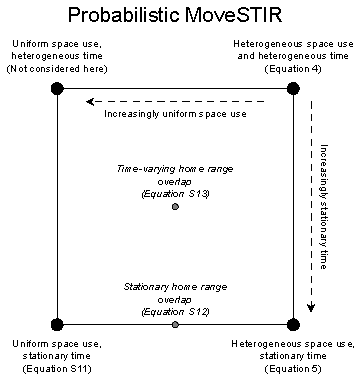
\includegraphics[width=\textwidth]{figures/conceptual_figure_pmovestir.pdf}
    \caption{Conceptual figure for PMoveSTIR}
	\label{fig:square}
\end{figure}

\begin{figure}
    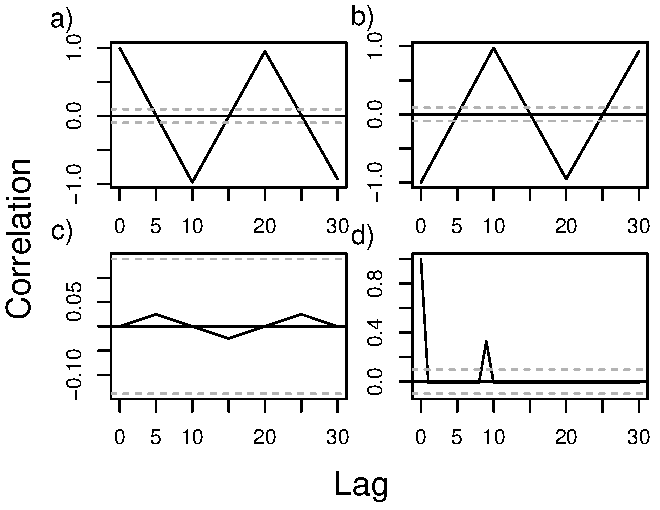
\includegraphics[width=\textwidth]{figures/example_xcorrs.pdf}
    \caption{Variation in cross-correlation values for different combinations of position histories}
	\label{fig:xcorrs}
\end{figure}

\begin{figure}
    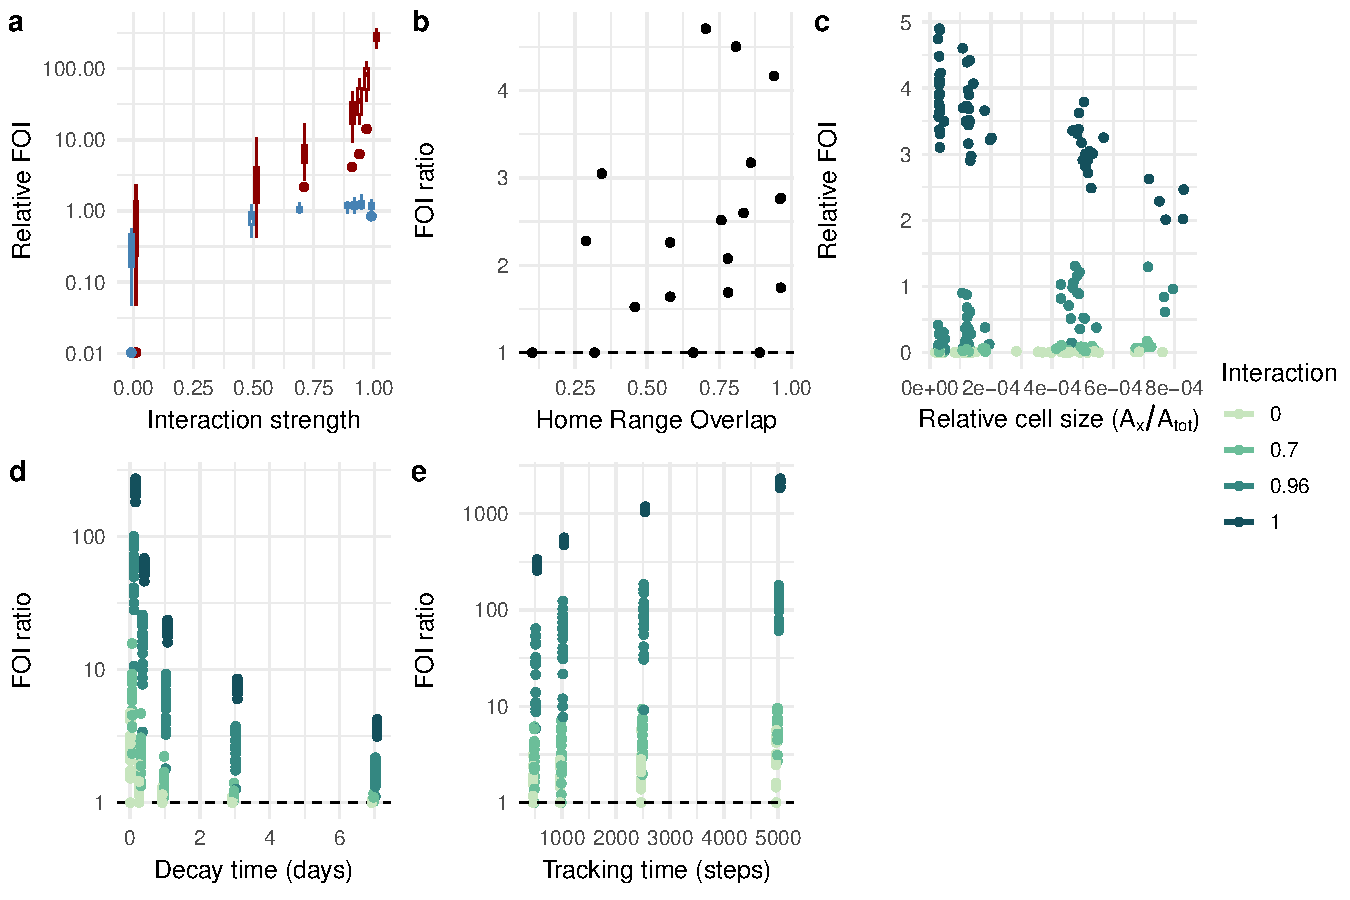
\includegraphics[width=\textwidth]{figures/sim_results.pdf}
    \caption{Analysis of simulated movement data show how the force of infection varies depending on movement processes, namely the strength of attraction between individuals, and how the estimated FOI depends on epidemiological parameters such as the decay rate and threshold distance}
	\label{fig:simresults}
\end{figure}

% \begin{figure}
%     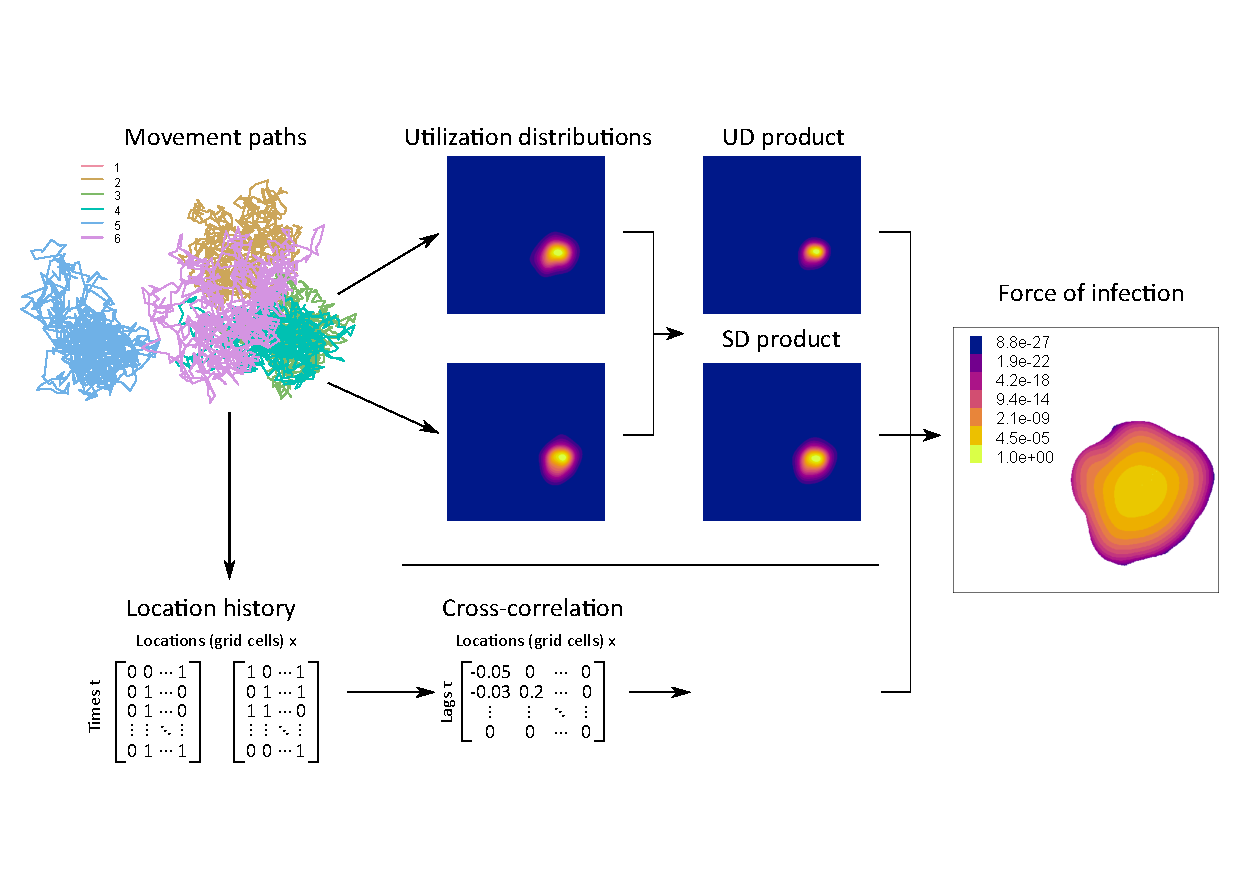
\includegraphics[width=\textwidth]{figures/steps_diagram.pdf}
%     \caption{Process to estimate pairwise FOIs using the PMoveSTIR framework, assuming stationary utilization distributions}
% 	\label{fig:steps}
% \end{figure}

\begin{figure}
     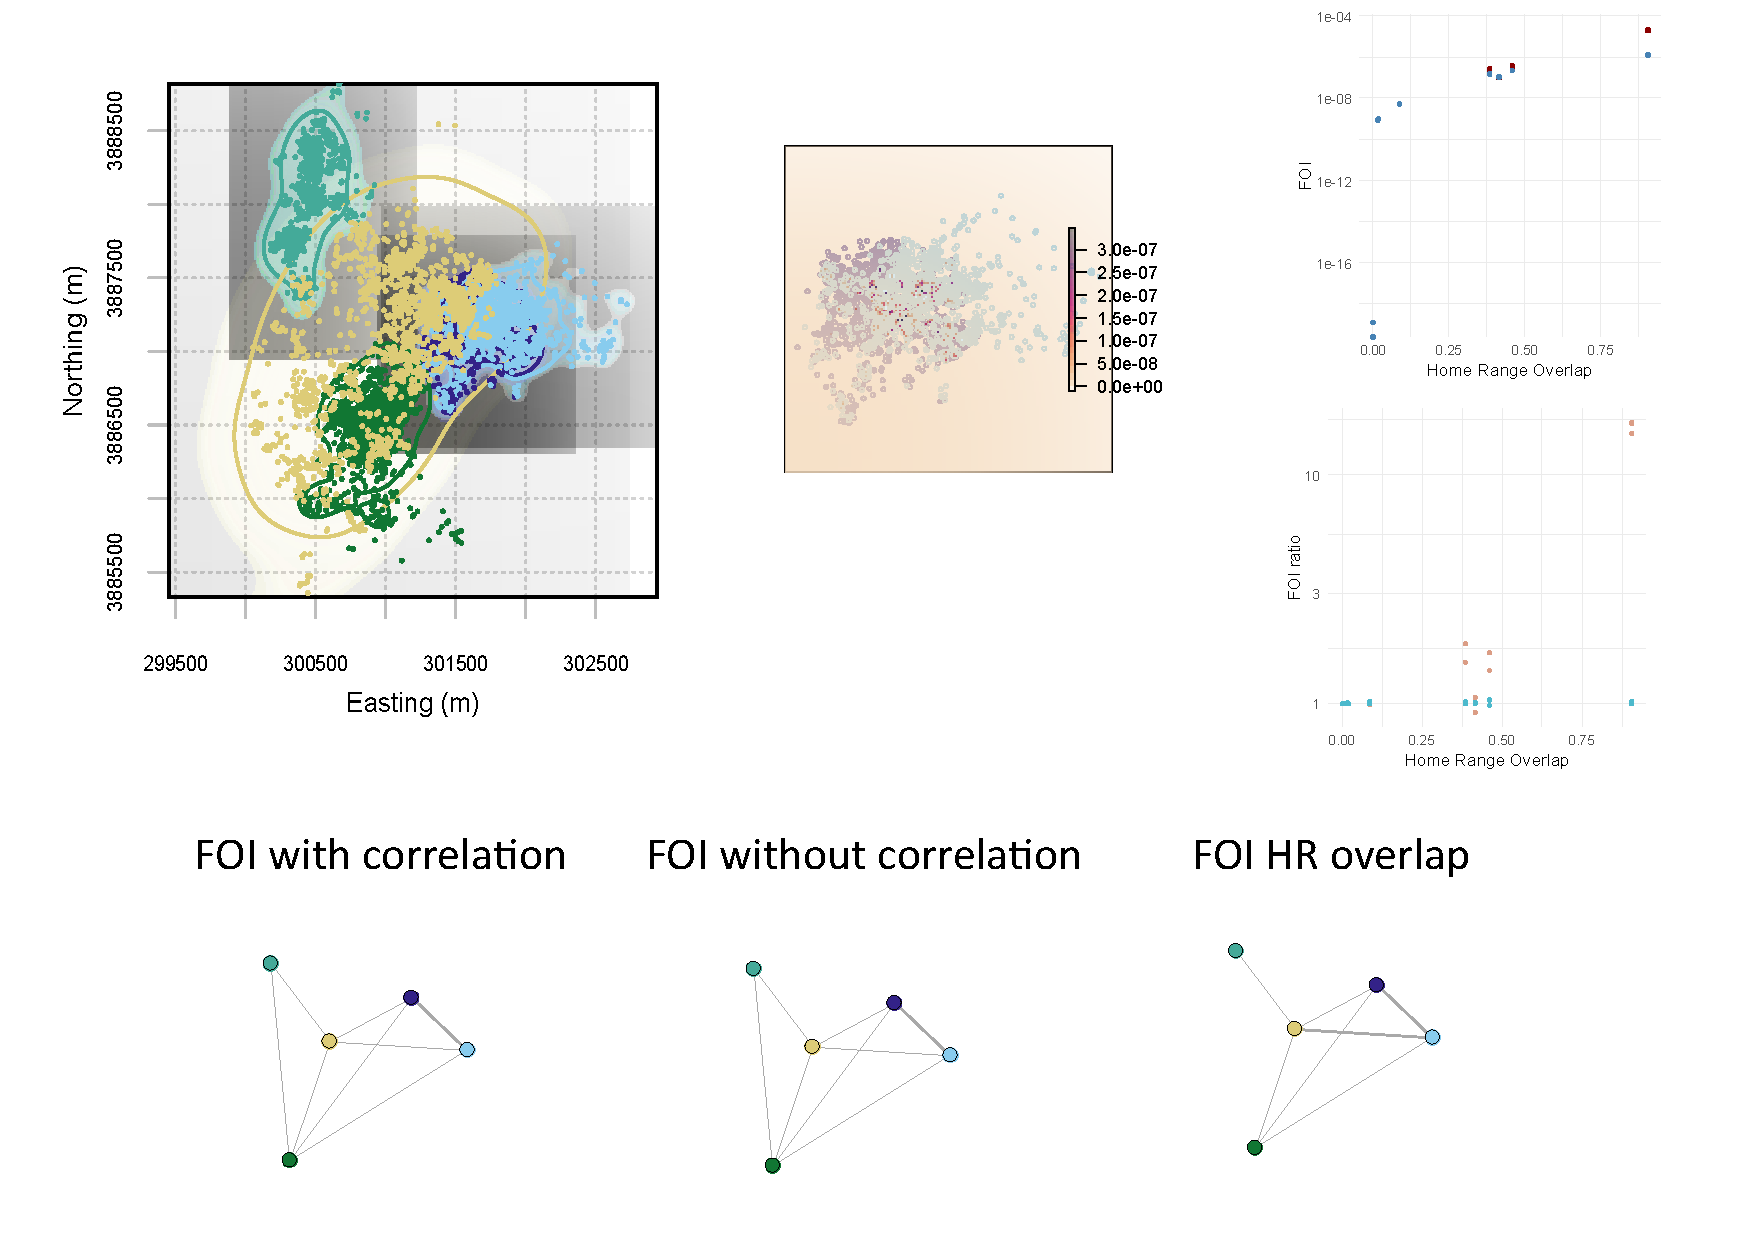
\includegraphics[width=\textwidth]{figures/deer_results.pdf}
    \caption{Empirical FOI estimates from tracking data of white-tailed deer}
	\label{fig:empiricalres}
\end{figure}


\end{document}
